\documentclass{article}
\usepackage{amsmath}
\usepackage{bm}
\usepackage{xcolor}
\usepackage{tikz}
\usetikzlibrary{shapes.geometric, arrows}
\usepackage{amssymb}
\begin{document}
	\title{Reinforcement Learning}
	\author{Tateyama Kaoru}
	\maketitle
\section{Continous RL}
Two pratical ways to impliment continous RL algorithm are discretization and modeling RL.
\subsection{Discretization}
We can discretize state space and action space so we'll turn the problem as we do in discretized case.But a clear downside of discretization is that when we have a lot of states and actions,the time complexity to impliment this algorithm will goes up really quickly.For example,say we need n parameters to determine a stete and m parameters to determine an action,now we have k states in total so to fully solve the system,the time complexity for states and actions will be $k^n$ and $k^m$ respectively.If we discretize the system into too many pieces,we have a large k resulting in unacceptable time complexity.
\subsection{Modelinig RL}
In this part,the approach is that we will set up a model for RL.A model means a mapping $S\times A\rightarrow S$,where $S$ denotes the state space and $A$ denotes the action space.The image of this mapping can be a fixed value or a random variable up to whether we're building a deterministic or stochastic model.
\begin{center}
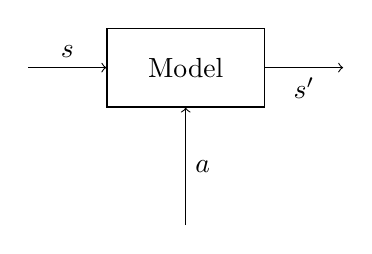
\begin{tikzpicture}
	\node[draw, rectangle, minimum width=2cm, minimum height=1cm] (box) at (0,0) {Model};
	\draw[->] (-2,0) -- (box) node[midway, above] {$s$};
	\draw[->] (0,-2) -- (box) node[midway, right] {$a$};
	\draw[->] (box) -- (2,0) node[midway, below] {$s'$};
	\node at (0, 0){};
\end{tikzpicture}
\end{center}
\textcolor{orange}{For the sake of convenience,still,we discretize actions}.To fit the model,we collect data by human control or other approaches and gather them together
\vspace{2\baselineskip}
\begin{align*}
	s^{(1)}_0\overset{\;\;a^{(1)}_0}{\longrightarrow}s^{(1)}_1\overset{\;\;a^{(1)}_1}{\longrightarrow}s^{(1)}_2\longrightarrow\cdots\overset{a^{(1)}_{T-1}}{\longrightarrow}s^{(1)}_T\\ 
\end{align*}
\[\vdots\]
\begin{align*}
	s^{(m)}_0\overset{\;\;a^{(m)}_0}{\longrightarrow}s^{(m)}_1\overset{\;\;a^{(m)}_1}{\longrightarrow}s^{(m)}_2\longrightarrow\cdots\overset{a^{(m)}_{T-1}}{\longrightarrow}s^{(m)}_T\\ 
\end{align*}
Then we'll use linear approximation to build the model.
\subsection{Deterministic}
We build the model by setting$$\textcolor{red}{s_{t+1}=As_t+Ba_t}$$where $s_{t+1}$ represents the state at step $t+1$ and $s_t$ and $a_t$ represent state and action taken at step $t$.A and B are matrixes.
\subsection{Stochastic}
We tend not to build too complicated stochastic model for RL,so we just put$$\textcolor{red}{s_{t+1}=As_t+Ba_t+w_t}$$where $w_t\sim N(0,\Sigma)$.A and B are matrixes.

The optimization goal are the same$$\textcolor{red}{\underset{A,B}{min}\sum_{i=1}^{m}\sum_{t=0}^{T}||s^{(i)}_{t+1}-(As^{(i)}_t+Ba^{(i)}_t)||^2}$$
Now we will set model for $V(s)$.We define $\phi(s)$ to be a vector function of $s$ and set$$\textcolor{red}{V^{*}(s)=\theta^{T}\phi(s)}$$We need to generate data set of $(s,V^{*}(s))$ so that we can fit the above equation.To do this,we sample $\{s^{(1)},s^{(2)}\cdots s^{(m)}\}$ randomly and impliment the fowllowing looop(called fitted value iteration)
\begin{align*}
	Loop\\ \{
	 &for\;i=1,2\cdots m\\ \{
	&\quad\quad for\;a_j\;in\;action\;space\;A\\ &\quad\{\\
	&\qquad create \;set\;\{s_{j1}',s_{j2}'\cdots s_{jk}'\}\sim {P_s^{(i)}a_j}\\
	&\quad\qquad let\;\textcolor{blue}{q(a_j)=\frac{1}{k}\sum_{l=1}^{k}[R(s^{(i)})+\gamma V(s_{jl}')]}\\&\quad\}\\&\qquad let\; \textcolor{orange}{y^{(i)}=\underset{a}{max}\;q(a)}\\&\quad
\}\\&\}
\end{align*}
The loop will end until outputs will live under tolerance.The blue part is simulating$$R(s)+\gamma\sum P_{s^{(i)}a}V(s^{(i)})$$and the orange part is simlulating$$\underset{a}{max}\;[R(s)+\gamma\sum P_{s^{(i)}a}V(s^{(i)})]$$When we go through the loop for many rounds enough,$y^{(i)}$ will be reasonably close to $V^{*}(s^{(i)})$.Therefore,instead,we will use $(s^{(i)},y^{(i)})$ to fit$$V^{*}(s)=\theta^T\phi(s)$$The optimization goal is nothing different from what we have in linear regression$$\underset{\theta}{min}\;\frac{1}{2}\sum_{i=1}^{m}(y^{(i)}-\theta^T\phi(s^{(i)}))^2$$
When we've done everything about fitting,we can determine the optimal policy via$$\pi^*(s)=arg\underset{a}{max}\;E_{s'\sim P_{s,a}}[V^*(s')]$$where we've already known how to calculate $V^*(s')\;\forall\;s'\;\in S$
\section{Generalized Reward}
\subsection{State Action Reward}
In a lot of occasions,Reward function is also dependent of action but not only state.Formally,we say Reward function R is a mapping$$R:S\times A\rightarrow \mathbb{R}$$Now Bellman's equation should be$$\textcolor{red}{V^*(s)=\underset{a}{max}[R(s,a)+\gamma\sum P_{s,a}(s')V^*(s')]}$$Almost identical to common Bellman's equation except that the optimal goal is added up with a new term.
\subsection{Finite Horizon MDP}
We now consider a MDP where the machine works in given and finite steps.It doesn't try to get to destination as soon as possible but tries to get more profit in given time or steps.Therefore,we don't need penalty constant $\gamma$ here and the payoff is now$$\sum_{t=1}^{T}R(s_t,a_t)$$
Since we have only finite steps,the value function $V(s)$ and policy $\pi(s)$ will also depend on step $t$ and we change the notation into $V_t(s)$ and $\pi_t(s)$.The optimazation goal is
\begin{align*}
	&\textcolor{red}{V^*_t(s)=\underset{a}{max}[R(s,a)+\sum^{s'}P_{s,a}(s')V^*_{t+1}(s')]}\\
	&\textcolor{red}{\pi^*_t(s)=\underset{a}{argmax}[R(s,a)+\sum^{s'}P_{s,a}(s')V^*_{t+1}(s')]}
\end{align*}
With initial condiction$$\textcolor{red}{V^*_T(s)=\underset{a}{max}R(s,a)}$$We can slove $V^*_t(s)\;\forall\;t\;and\;s$ along solving the sequance$$V^*_T,V^*_{T-1}\cdots V^*_0$$Afterwards,it will be simple to solve optimal policy as well.
\section{Linear Quadratic Regularization}
A toy model for MDP is to set Rewad function and value function to be quadratic functions.Say $U$ and $V$ are semi-positive symmetric matrixes.Let$$\textcolor{red}{R(s,a)=-(s^TUs+a^TVa)}$$and consider linear model$$\textcolor{red}{s_{t+1}=As_t+Ba_t+w_t}$$where $w_t\sim N(0,\Sigma)$,with $\Sigma$ being covariance matrix.We will also assume that$$\textcolor{red}{V^*_{t+1}(s_{t+1})=s^T_{t+1}\Phi_{t+1}s_{t+1}+\Psi_{t+1}}$$We can always take $\Phi_{t+1}$ to be symmetric as we only consider quadratic term.Still,we consider finite horizon case,so optimization goal is$$\textcolor{blue}{V^*_t(s_t)=\underset{a_t}{max}\{-s^T_tUs_t-a_tVa_t+E_{s_{t+1}\sim N(As_t+Ba_t+w_t)}[s_{t+1}^T\Phi_{t+1}s_{t+1}+\Psi_{t+1}]\}}$$with$$\textcolor{blue}{V^*_T(S_T)=\underset{a_T}{max}\;R(s_T,a_T)=-s^T_TUs_T}$$as $-a^T_TVa_T\le0$.Now we substitue $s_{t+1}$ in the Bellman's equation and note that $E[w_t]=0$ so we tansform the optimization goal into $\underset{a_t}{max}\;K(a_t)$,where$$K(a_t)=s^T_tA^T\Phi_{t+1}Ba_t+a^T_tB^T\Phi_{t+1}As_t+a^T_tB^T\Phi_{t+1}Ba_t$$Take derivative with respect to $a_t$ and set it to be zero so we obtain$$\textcolor{red}{a_t=-(B^T\Phi_{t+1}B-V)^{-1}B^T\Phi_{t+1}As_t\equiv L_ts_t}$$substitute in $V^*_t(s_t)$,we get that$$\textcolor{red}{V^*_t(s_t)=s^T_t\Phi_ts_t+\Psi_t}$$where
$$\textcolor{red}{\Phi_t=A^T(\Phi_{t+1}-\Phi_{t+1}B(B^T\Phi_{t+1}B-V)^{-1}B^T\Phi_{t+1})A-U}$$
$$\textcolor{red}{\Psi_t=\Psi_{t+1}+tr(\Sigma\Phi_{t+1})}$$
one can check that $\Phi_t$ is also symmetric.
\end{document}